\section{Installation}
\label{sec:installation}

In this section, we will describe the various ways that one can build \pkg{pbdPROF} and link it with MPI-using \proglang{R} packages.  For installation troubleshooting, see \instdebug.


\subsection[System Requirements]{System Requirements}
\label{sec:system_requirements}

The \pkg{pbdPROF} package requires an MPI installation, such as OpenMPI or 
MS-MPI.  Additionally, the package is basically useless without some kind of 
MPI-using \proglang{R} package, such 
as \pkg{pbdMPI}~\citep{Chen2012pbdMPIpackage} or \pkg{Rmpi}~\citep{Yu2002}.
For information regarding how to install MPI or \pkg{pbdMPI}, please see the 
\pkg{pbdMPI} vignette~\citep{Chen2012pbdMPIvignette} or the pbdR website 
\url{http://r-pbd.org/install}.


\subsection{The Big Picture}

Before pressing on, let us stop to take a moment and understand the ``big 
picture'' here. The following sections will contain \emph{more than sufficient} 
detail, to the point where it would be easy to lose sight of the proverbial 
forest for the trees.

For the remainder of this document, we will be providing information for two 
fairly distinct groups of people:  \proglang{R}-level MPI package developers, 
and \proglang{C}/\proglang{Fortran}-level MPI package developers.  If you are 
in the former category, then the use of this package is a bit simpler for you.  
All you need to do is get \pkg{pbdPROF} installed and reinstall your MPI-using 
package of choice (\pkg{pbdMPI}, \pkg{Rmpi}, etc. \dots).  Each package that 
directly uses MPI (packages produced by developers in the latter category) will 
have to explicitly support \pkg{pbdPROF} (or the reader will have to get 
his/her hands dirty in another developer's makefiles --- an unpleasant 
business).  It is worth nothing here that there are instructions in this 
document for how a developer of the second kind could explicitly add 
\pkg{pbdPROF} support to his/her package.
  
So why the need to reinstall things?  It boils down to how the profilers 
actually work.  Under normal circumstances, a user writes some \proglang{R} code 
from an MPI-using package (e.g., \code{allreduce(x)} from \pkg{pbdMPI}, 
\code{mpi.allreduce(x, type=2)} from \pkg{Rmpi}, etc. \dots).
%\begin{figure}[h]
%  \centering
%  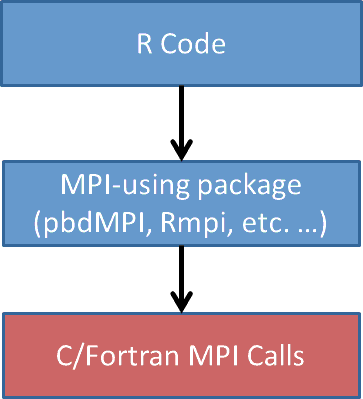
\includegraphics[scale=.4]{include/pics/mpi_normal}
%  \caption{Without a Profiler}
%  \label{fig:normalmpi}
%\end{figure}

\begin{figure}
  \hspace{0.2cm}
  \begin{subfigure}[b]{0.3\textwidth}
    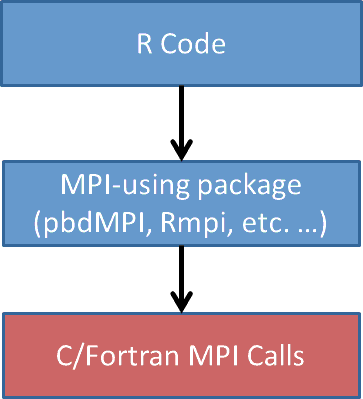
\includegraphics[width=0.9\textwidth]{include/pics/mpi_normal}
    \caption{Without a Profiler}
    \label{fig:normalmpi}
  \end{subfigure}
  \hspace{0.3cm}
  \begin{subfigure}[b]{0.3\textwidth}
    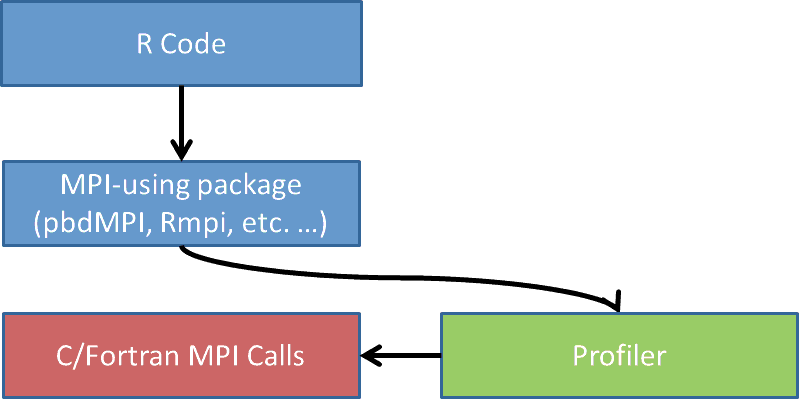
\includegraphics[width=2.0\textwidth]{include/pics/mpi_profiler}
    \caption{With the Profiler}
    \label{fig:profmpi}
  \end{subfigure}
\end{figure}

This then makes a call to some \proglang{C} or \proglang{Fortran} code which 
directly interfaces with MPI.  You can see this pictures in 
\figref{fig:normalmpi}.  When you use a profiler, you instead hijack the 
calls to MPI from the \proglang{C}/\proglang{Fortran} code so that some 
metadata can be stored about MPI usage.

%\begin{figure}[h]
%   \centering
%  \hspace*{6.1cm}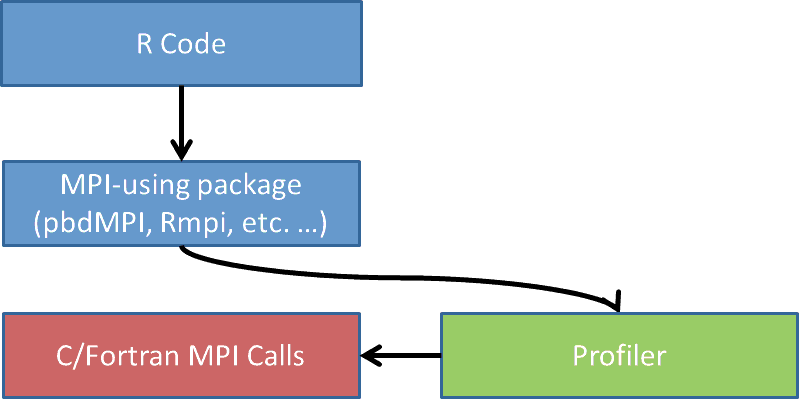
\includegraphics[scale=.4]{include/pics/mpi_profiler}
%  \caption{With the Profiler}
%  \label{fig:profmpi}
%\end{figure}

This process is represented in \figref{fig:profmpi}.  Hopefully it should 
be clear what, and when, something should be reinstalled.  For the sake of 
completion, we summarize the possibilities below:

To \emph{enable} MPI profiling:
\begin{enumerate}
  \item install \pkg{pbdPROF}
  \item reinstall an MPI-using package and link it with \pkg{pbdPROF}
  \item write and execute your MPI-using \proglang{R} code as normal
  \item use the \pkg{pbdPROF} utilities \code{read.prof()}, etc. 
for interpreting profiling results
\end{enumerate}
To \emph{disable} MPI profiling:
\begin{enumerate}
  \item reinstall any MPI-using package that was linked it with \pkg{pbdPROF}, 
and this time \emph{do not} link with \pkg{pbdPROF}
\end{enumerate}



% \subsection{Choice of Profiler}
% 
% {\color{red}
% Regardless of whether \pkg{fpmpi}, \pkg{mpiP}, or \pkg{TAU} is used, we 
% strongly recommend adding \code{CPPFLAGS="-fPIC"} at the \code{configure} step.
% }


\subsection{Installing pbdPROF with fpmpi}
\label{sec:fpmpi}

We can install \pkg{pbdPROF} using the internal \pkg{fpmpi} library via
\begin{Command}
R CMD INSTALL pbdPROF_0.1-0.tar.gz
\end{Command}
By default, this compiles \code{pbdPROF/src/fpmpi/*} of the \pkg{pbdPROF} source, 
generates a static library \code{libfpmpi.a}, and installs the library to
\code{pbdPROF/lib/} of the \pkg{pbdPROF} install. No shared library is generated 
or needed, so the directory
\code{pbdPROF/libs/} is empty, i.e., there is no need to build \code{pbdPROF.so}.
The linking argument is saved in \code{Makeconf} and installed to
\code{pbdPROF/etc/} for later use by other packages, such as \pkg{pbdMPI} or \pkg{Rmpi}.


However, if we choose, we can link with an external \pkg{fpmpi} library, via
\begin{Command}
R CMD INSTALL pbdPROF_0.1-0.tar.gz \
  --configure-args="--with-fpmpi='/path_to_fpmpi/lib/libfpmpi.a'"
\end{Command}
or
\begin{Command}
R CMD INSTALL pbdPROF_0.1-0.tar.gz \
  --configure-args="--with-fpmpi='-L/path_to_fpmpi/lib -lfpmpi'"
\end{Command}
Or the conventional method in R console
\begin{Command}
install.packages("pbdPROF", configure.args=c("--with-fpmpi=/path/to/your/fpmpi/lib/libfpmpi.a"))
\end{Command}
Or
\begin{Command}
install.packages("pbdPROF", configure.args=c("--with-fpmpi=-L/path/to/your/fpmpi/lib -lfpmpi"))
\end{Command}
Since \pkg{fpmpi} only builds a static library \code{libfpmpi.a}, there is
no difference between these two installations of \pkg{pbdPROF}.
This only provides the linking arguments, either
\code{/path_to_fpmpi/lib/libfpmpi.a} or
\code{-L/path_to_fpmpi/lib -lfpmpi},
which is saved in \code{Makeconf} and installed to
\code{pbdPROF/etc/} for later use by other packages, such as \pkg{pbdMPI} or \pkg{Rmpi}.


\subsubsection{Linking \pkg{pbdMPI} with pbdPROF}
\label{sec:pbdMPI}

Reinstall \pkg{pbdMPI} via
\begin{Command}
R CMD INSTALL pbdMPI_1.0-0.tar.gz --configure-args="--enable-pbdPROF"
\end{Command}
Package developers who are directly interfacing with MPI functions
(via \proglang{C} or \proglang{Fortran}) 
should note that \code{pbdMPI/R/get_conf.r} and \code{pbdMPI/R/get_lib.r} are
utilized in \code{pbdMPI/configure.ac}
(used to generate \code{pbdMPI/configure})
to determine an
appropriate linking flag \code{PROF_LDFLAGS} based on preset flags in
\code{pbdPROF/etc/Makeconf}.

If the internal library is used in \pkg{pbdPROF},
then the path to \code{pbdPROF/lib/libfpmpi.a} is set in the flag
\code{PKG_LIBS} of \code{pbdMPI/src/Makevars.in}.
If the external library is used in \pkg{pbdPROF},
then the linking arguments either \code{/path_to_fpmpi/lib/libfpmpi.a} or
\code{-L/path_to_fpmpi/lib -lfpmpi} is set
in the flag \code{PKG_LIBS} of \code{pbdMPI/src/Makevars.in}.
Therefore, the \pkg{pbdMPI} can be intercepted by the \pkg{fpmpi} library
when MPI function calls are evoked.

No mater which library is used, internal or external, the \code{PROF_LDFLAGS}
in \code{pbdMPI/etc/Makefile} provides the linking information to the
profiling library. It is also used in \code{PKG_LIBS}, which will be
exported to other \proglang{pbdR} packages at installation via the flag
\code{SPMD_LDFLAGS}.  Therefore there is no need for additional flags in
\code{R CMD INSTALL} when reinstalling packages for profiling.



\subsubsection{Linking \pkg{pbdBASE} with pbdPROF}
\label{sec:pbdBASE}

For further profiling, such as \pkg{pbdBASE}~\citep{Schmidt2012pbdBASEpackage}, one may
reinstall the package, via
\begin{Command}
R CMD INSTALL pbdBASE_0.2-2.tar.gz
\end{Command}
There is no need to provide any flag since \pkg{pbdMPI/etc/Makefile} has the
information and installation of \pkg{pbdBASE} already considers it.
Note that since both packages (\pkg{pbdMPI} and \pkg{pbdBASE})
have MPI-using \proglang{C}/\proglang{Fortran} functions involved, it
is necessary to link with \pkg{pbdPROF} in order to profile communications
evoked by the package.



\subsubsection{Linking \pkg{Rmpi} with pbdPROF}
\label{sec:Rmpi}

Reinstall \pkg{Rmpi} via
\begin{Command}
wget https://github.com/snoweye/Rmpi_PROF/archive/master.zip
unzip master.zip
mv Rmpi_PROF-master Rmpi
find ./Rmpi -type f -perm 777 -print -exec chmod 644 {} \;
find ./Rmpi -type d -perm 777 -print -exec chmod 755 {} \;
chmod 755 ./Rmpi/configure
chmod 755 ./Rmpi/cleanup
chmod 755 ./Rmpi/inst/*.sh
R CMD build --no-resave-data Rmpi
R CMD INSTALL Rmpi_0.6-6.tar.gz --configure-args="--enable-pbdPROF"
\end{Command}
Note that {\color{red} 0.6-6} is not an official release of \pkg{Rmpi}.
It is a modified version of 0.6-3 and it is currently available at
\url{https://github.com/snoweye/Rmpi_PROF}.  The authors of \pkg{Rmpi} have plans 
to eventually incorporate these changes, but this can be used as a temporary 
measure.






\subsection{Installing pbdPROF with mpiP}
\label{sec:mpiP}

We have to install \pkg{mpiP} externally from its source code to use it in
\pkg{pbdPROF}. We can install \pkg{pbdPROF} using the external \pkg{mpiP} library via
\begin{Command}
R CMD INSTALL pbdPROF_0.2-0.tar.gz --configure-args="--with-mpiP='/path/to/your/mpiP/lib/libmpiP.a' "
\end{Command}
Or
\begin{Command}
R CMD INSTALL pbdPROF_0.2-0.tar.gz --configure-args="--with-mpiP='-L/path/to/your/mpiP/lib lmpiP' "
\end{Command}
Or the conventional method in R console
\begin{Command}
install.packages("pbdPROF", configure.args=c("--with-mpiP=/path/to/your/mpiP/lib/libmpiP.a"))
\end{Command}
Or
\begin{Command}
install.packages("pbdPROF", configure.args=c("--with-mpiP=-L/path/to/your/mpiP/lib -lmpiP"))
\end{Command}


\code{pbdPROF/libs/} is empty, i.e., there is no need to build \code{pbdPROF.so}.
The linking argument is saved in \code{Makeconf} and installed to
\code{pbdPROF/etc/} for later use by other packages, such as \pkg{pbdMPI} or \pkg{Rmpi}.
Since \pkg{mpiP} has external dependency \code{libfpmpi.a} on libunwind so while installing 
\pkg{mpiP} you are suggested to use the below command while configuring \pkg{mpiP}.
This only provides the linking arguments, either
\begin{Code}
./configure --disable-libunwind CPPFLAGS="-fPIC -I/usr/lib/openmpi/include" LDFLAGS="-L/usr/lib/openmpi/lib -lmpi"
\end{Code}
since one has changed the linking so need to reinstall packages depend on \pkg{Code}pbdPROF



\subsubsection{Linking \pkg{pbdMPI} with pbdPROF}
\label{sec:pbdMPI}

Reinstall \pkg{pbdMPI} via
\begin{Command}
R CMD INSTALL pbdMPI_1.0-0.tar.gz --configure-args="--enable-pbdPROF"
\end{Command}
Package developers who are directly interfacing with MPI functions
(via \proglang{C} or \proglang{Fortran}) 
should note that \code{pbdMPI/R/get_conf.r} and \code{pbdMPI/R/get_lib.r} are
utilized in \code{pbdMPI/configure.ac}
(used to generate \code{pbdMPI/configure})
to determine an
appropriate linking flag \code{PROF_LDFLAGS} based on preset flags in
\code{pbdPROF/etc/Makeconf}.

If your pbdMPI is correctly installed with all correct linking you will have the screenshot just similar to below output 
during installation of \pkg{pbdMPI} or else you might get error 
\begin{Output}
******************* Results of pbdMPI package configure *****************
 
>> TMP_INC = /usr/local/include
>> TMP_LIB = /usr/local/lib
>> MPI_ROOT = 
>> MPITYPE = OPENMPI
>> MPI_INCLUDE_PATH = /usr/local/include
>> MPI_LIBPATH = /usr/local/lib
>> MPI_LIBS =  -lutil -lpthread
>> MPI_DEFS = -DMPI2
>> MPI_INCL2 = 
>> PKG_CPPFLAGS = -I/usr/local/include  -DMPI2 -DOPENMPI
>> PKG_LIBS = /home/g/Documents/new_life/lib/libmpiP.a -L/usr/local/lib -lmpi  -lutil -lpthread
>> PROF_LDFLAGS = /home/g/Documents/new_life/lib/libmpiP.a
 
*************************************************************************

\end{Output}

No mater which library is used, internal or external, the \code{PROF_LDFLAGS}
in \code{pbdMPI/etc/Makefile} provides the linking information to the
profiling library. It is also used in \code{PKG_LIBS}, which will be
exported to other \proglang{pbdR} packages at installation via the flag
\code{SPMD_LDFLAGS}.  Therefore there is no need for additional flags in
\code{R CMD INSTALL} when reinstalling packages for profiling.


\subsubsection{Linking \pkg{pbdBASE} with pbdPROF}
\label{sec:pbdBASE}

For further profiling, such as \pkg{pbdBASE}~\citep{Schmidt2012pbdBASEpackage}, one may
reinstall the package, via
\begin{Command}
R CMD INSTALL pbdBASE_0.2-2.tar.gz
\end{Command}
There is no need to provide any flag since \pkg{pbdMPI/etc/Makefile} has the
information and installation of \pkg{pbdBASE} already considers it.
Note that since both packages (\pkg{pbdMPI} and \pkg{pbdBASE})
have MPI-using \proglang{C}/\proglang{Fortran} functions involved, it
is necessary to link with \pkg{pbdPROF} in order to profile communications
evoked by the package.


\subsubsection{Linking \pkg{Rmpi} with pbdPROF}
\label{sec:Rmpi}

Reinstall \pkg{Rmpi} via
\begin{Command}
wget https://github.com/snoweye/Rmpi_PROF/archive/master.zip
unzip master.zip
mv Rmpi_PROF-master Rmpi
find ./Rmpi -type f -perm 777 -print -exec chmod 644 {} \;
find ./Rmpi -type d -perm 777 -print -exec chmod 755 {} \;
chmod 755 ./Rmpi/configure
chmod 755 ./Rmpi/cleanup
chmod 755 ./Rmpi/inst/*.sh
R CMD build --no-resave-data Rmpi
R CMD INSTALL Rmpi_0.6-4.tar.gz --configure-args="--enable-pbdPROF"
\end{Command}
Note that {\color{red} 0.6-4} is not an official release of \pkg{Rmpi}.
It is a modified version of 0.6-3 and it is currently available at
\url{https://github.com/snoweye/Rmpi_PROF}.  The authors of \pkg{Rmpi} have plans 
to eventually incorporate these changes, but this can be used as a temporary 
measure.
